\documentclass[10pt]{beamer}

% Lecture 05, part 1 of 2: the ideas behind the transformer, in about 55 minutes.  Part 2 is the
% notebook (notebooks/archive/06_transformers_old.ipynb).  This deck is a simplified version of
% self_attention_and_transformers.tex in the same folder: one idea per slide, and it reuses that
% deck's figures in images/ (made by make_figures.py; images/SOURCES.md says what each shows).
% Numbers copied from that deck carry the same provenance as there.

\usepackage[T1]{fontenc}

\usetheme{metropolis}

\usepackage{graphicx}
\graphicspath{{images/}}
\usepackage{amsmath, amssymb, amsthm}
\usepackage{mathtools}
\usepackage{bm}
\usepackage{booktabs}
\usepackage{array}
\usepackage{tikz}
\usetikzlibrary{positioning, arrows.meta, calc, fit, backgrounds}
\usepackage{listings}
\usepackage{xcolor}
\usepackage[numbers,square]{natbib}
\usepackage[most]{tcolorbox}
\usepackage{tabularx}
\usepackage{colortbl}
\usepackage{xurl}
\definecolor{codebg}{RGB}{245,245,245}
\definecolor{codeframe}{RGB}{180,180,180}
\definecolor{boxbg}{RGB}{235,245,255}
\definecolor{boxframe}{RGB}{70,130,180}
\definecolor{ctrl}{HTML}{EB6834}   % P.ORANGE, as in the figures
\definecolor{posneg}{HTML}{2A78D6} % P.BLUE: negative values on a signed colour scale

\lstdefinestyle{pytorch}{
  language=Python,
  basicstyle=\ttfamily\scriptsize,
  keywordstyle=\color{blue!70!black}\bfseries,
  stringstyle=\color{green!50!black},
  commentstyle=\color{gray}\itshape,
  showstringspaces=false,
  breaklines=true,
  columns=fullflexible,
  keepspaces=true,
  backgroundcolor=\color{codebg},
  frame=single,
  rulecolor=\color{codeframe},
  framesep=4pt,
  xleftmargin=4pt,
  xrightmargin=4pt,
}
\lstset{style=pytorch}
\definecolor{outbg}{RGB}{238,247,238}
\definecolor{outframe}{RGB}{140,180,140}
\lstdefinestyle{output}{style=pytorch, language={}, backgroundcolor=\color{outbg}, rulecolor=\color{outframe}, aboveskip=0pt}

\title{Self-Attention and Transformers}
\subtitle{Part 1: the ideas}
\author{Enrique Zuazua, Daniel L\'opez Montero}
\date{Winter 2026}
\institute{Mathematical Foundations of Control and Machine Learning\\FAU Erlangen-N\"urnberg}

% --- Math shortcuts --------------------------------------------------------
\newcommand{\R}{\mathbb{R}}
\newcommand{\E}{\mathbb{E}}
\newcommand{\Vocab}{\mathcal{V}}   % the vocabulary: the finite set of tokens
\newcommand{\ctrl}[1]{\textcolor{ctrl}{#1}}
\DeclareMathOperator{\Var}{Var}
\DeclareMathOperator{\softmax}{softmax}
\DeclareMathOperator{\score}{score}
\DeclareMathOperator{\Attention}{Attention}
\DeclareMathOperator{\MLP}{MLP}
\DeclareMathOperator{\LN}{LN}
\DeclareMathOperator*{\argmax}{arg\,max}

% --- Boxes -------------------------------------------------------------------
\newtcolorbox{mathbox}[2][]{
  colback=boxbg, colframe=boxframe, boxrule=0.2pt, arc=2pt,
  left=4pt, right=4pt, top=2pt, bottom=2pt,
  title=\textbf{#2}, fonttitle=\small, coltitle=white, colbacktitle=boxframe,
  halign=left, #1}
\definecolor{asmbg}{RGB}{245,240,251}
\definecolor{asmframe}{RGB}{125,90,165}
\tcbset{assumption/.style={colback=asmbg, colframe=asmframe, colbacktitle=asmframe}}
% \takeaway{...}: the one sentence to remember from a slide, at its foot.
\newcommand{\takeaway}[1]{%
  \par\medskip
  \begin{tcolorbox}[enhanced, colback=ctrl!8, colframe=ctrl, boxrule=0pt, leftrule=2.5pt, arc=0pt,
      left=5pt, right=5pt, top=2.5pt, bottom=2.5pt, before skip=0pt, after skip=0pt]
  \small #1
  \end{tcolorbox}}

% --- The pipeline: text -> tokens -> vectors -> transformer -> next token ---------
% \pipeline{s1}{s2}{s3}{s4}{s5}: each argument is a style for one box, "on" to highlight it.
% It opens the lecture and is drawn on every section page with that section's boxes highlighted.
\tikzset{on/.style={draw=ctrl, fill=ctrl!14, line width=0.9pt}}
\newcommand{\pipeline}[5]{%
\begin{tikzpicture}[x=1cm, y=1cm, font=\scriptsize, >=Stealth,
    st/.style={draw=boxframe, fill=boxbg, rounded corners=2pt, align=center,
               minimum width=2.05cm, minimum height=1.05cm, inner sep=2pt},
    ar/.style={->, boxframe, line width=0.7pt}]
  \node[st, #1] (a) at (0,0)     {\textbf{Text}\\[1pt] \texttt{The dog bites}};
  \node[st, #2] (b) at (2.75,0)  {\textbf{Tokens}\\[1pt] $i_1,\dots,i_n\in\Vocab$};
  \node[st, #3] (c) at (5.5,0)   {\textbf{Vectors}\\[1pt] $x_t=e_{i_t}+p_t$};
  \node[st, #4, minimum width=2.3cm] (d) at (8.35,0) {\textbf{Transformer}\\[1pt] attention + MLP\\ $L$ times};
  \node[st, #5, minimum width=2.6cm] (e) at (11.4,0) {\textbf{Next token}\\[1pt] $p(i_{n+1}\mid i_1,\dots,i_n)$};
  \draw[ar] (a) -- (b);
  \draw[ar] (b) -- (c);
  \draw[ar] (c) -- (d);
  \draw[ar] (d) -- (e);
\end{tikzpicture}}
% The highlighted boxes of section k.
\newcommand{\pipelinefor}[1]{%
  \ifcase#1\relax \pipeline{}{}{}{}{}%
  \or \pipeline{}{}{}{on}{}%   1. why attention
  \or \pipeline{on}{on}{on}{}{}% 2. from text to vectors
  \or \pipeline{}{}{}{on}{}%   3. self-attention
  \or \pipeline{}{}{on}{on}{}% 4. word order: positions and the mask
  \or \pipeline{}{}{}{on}{on}% 5. the transformer and its training
  \else \pipeline{}{}{}{}{}\fi}

% \maskgrid{1}: a 5 x 5 grid of the weights alpha_ts that may be nonzero (row t, column s) under the
% causal mask; \maskgrid{0}: without it.
\newcommand{\maskgrid}[1]{%
  \begin{tikzpicture}[x=2.3mm, y=2.3mm]
    \foreach \row in {0,...,4} \foreach \col in {0,...,4} {
      \ifnum#1=1 \ifnum\col>\row \def\f{white}\else\def\f{boxframe!55}\fi \else \def\f{boxframe!55}\fi
      \filldraw[fill=\f, draw=black!25, line width=0.2pt] (\col,-\row) rectangle ++(1,-1);
    }
  \end{tikzpicture}}

\setbeamertemplate{section in toc}[sections numbered]
\setbeamertemplate{section page}{%
  \centering
  {\usebeamercolor[fg]{section title}\usebeamerfont{section title}\LARGE
   \insertsectionnumber.\ \insertsectionhead\par}
  \vspace{1.0cm}
  \resizebox{\linewidth}{!}{\pipelinefor{\insertsectionnumber}}\par}

\setbeamertemplate{bibliography item}[text]
\renewcommand{\bibsection}{}

% --- Bibliography database: written to the .bib on each compilation ------------
\begin{filecontents}[overwrite]{self_attention_and_transformers_part1.bib}
@inproceedings{bahdanau2015,
  author    = {Bahdanau, Dzmitry and Cho, Kyunghyun and Bengio, Yoshua},
  title     = {Neural Machine Translation by Jointly Learning to Align and Translate},
  booktitle = {International Conference on Learning Representations (ICLR)},
  year      = {2015},
  note      = {arXiv:1409.0473}
}

@article{bengio1994,
  author  = {Bengio, Yoshua and Simard, Patrice and Frasconi, Paolo},
  title   = {Learning Long-Term Dependencies with Gradient Descent Is Difficult},
  journal = {IEEE Transactions on Neural Networks},
  volume  = {5},
  number  = {2},
  pages   = {157--166},
  year    = {1994},
  doi     = {10.1109/72.279181}
}

@article{bengio2003,
  author  = {Bengio, Yoshua and Ducharme, R{\'e}jean and Vincent, Pascal and Jauvin, Christian},
  title   = {A Neural Probabilistic Language Model},
  journal = {Journal of Machine Learning Research},
  volume  = {3},
  pages   = {1137--1155},
  year    = {2003}
}

@inproceedings{devlin2019,
  author    = {Devlin, Jacob and Chang, Ming-Wei and Lee, Kenton and Toutanova, Kristina},
  title     = {{BERT}: Pre-training of Deep Bidirectional Transformers for Language Understanding},
  booktitle = {Proceedings of the 2019 Conference of the North American Chapter of the Association for Computational Linguistics (NAACL)},
  pages     = {4171--4186},
  year      = {2019},
  doi       = {10.18653/v1/N19-1423},
  note      = {arXiv:1810.04805}
}

@article{elman1990,
  author  = {Elman, Jeffrey L.},
  title   = {Finding Structure in Time},
  journal = {Cognitive Science},
  volume  = {14},
  number  = {2},
  pages   = {179--211},
  year    = {1990},
  doi     = {10.1207/s15516709cog1402_1}
}

@article{gage1994,
  author  = {Gage, Philip},
  title   = {A New Algorithm for Data Compression},
  journal = {The C Users Journal},
  volume  = {12},
  number  = {2},
  pages   = {23--38},
  month   = feb,
  year    = {1994}
}

@misc{graves2014,
  author = {Graves, Alex and Wayne, Greg and Danihelka, Ivo},
  title  = {Neural {T}uring Machines},
  year   = {2014},
  note   = {arXiv:1410.5401}
}

@article{hochreiter1997,
  author  = {Hochreiter, Sepp and Schmidhuber, J{\"u}rgen},
  title   = {Long Short-Term Memory},
  journal = {Neural Computation},
  volume  = {9},
  number  = {8},
  pages   = {1735--1780},
  year    = {1997},
  doi     = {10.1162/neco.1997.9.8.1735}
}

@misc{huang2022,
  author       = {Huang, Austin and Subramanian, Suraj and Sum, Jonathan and Almubarak, Khalid and Biderman, Stella},
  title        = {The Annotated Transformer},
  howpublished = {Web notebook, 2022 version of the original by A. Rush (2018)},
  year         = {2022},
  url          = {https://nlp.seas.harvard.edu/annotated-transformer/}
}

@inproceedings{luong2015,
  author    = {Luong, Thang and Pham, Hieu and Manning, Christopher D.},
  title     = {Effective Approaches to Attention-based Neural Machine Translation},
  booktitle = {Proceedings of the 2015 Conference on Empirical Methods in Natural Language Processing (EMNLP)},
  pages     = {1412--1421},
  year      = {2015},
  doi       = {10.18653/v1/D15-1166},
  note      = {arXiv:1508.04025}
}

@article{nadaraya1964,
  author  = {Nadaraya, E. A.},
  title   = {On Estimating Regression},
  journal = {Theory of Probability \& Its Applications},
  volume  = {9},
  number  = {1},
  pages   = {141--142},
  year    = {1964},
  doi     = {10.1137/1109020}
}

@techreport{radford2018,
  author      = {Radford, Alec and Narasimhan, Karthik and Salimans, Tim and Sutskever, Ilya},
  title       = {Improving Language Understanding by Generative Pre-Training},
  institution = {OpenAI},
  year        = {2018},
  url         = {https://cdn.openai.com/research-covers/language-unsupervised/language_understanding_paper.pdf}
}

@techreport{radford2019,
  author      = {Radford, Alec and Wu, Jeffrey and Child, Rewon and Luan, David and Amodei, Dario and Sutskever, Ilya},
  title       = {Language Models Are Unsupervised Multitask Learners},
  institution = {OpenAI},
  year        = {2019},
  url         = {https://cdn.openai.com/better-language-models/language_models_are_unsupervised_multitask_learners.pdf}
}

@inproceedings{rush2018,
  author    = {Rush, Alexander},
  title     = {The Annotated Transformer},
  booktitle = {Proceedings of Workshop for {NLP} Open Source Software ({NLP-OSS})},
  address   = {Melbourne, Australia},
  publisher = {Association for Computational Linguistics},
  pages     = {52--60},
  year      = {2018},
  doi       = {10.18653/v1/W18-2509}
}

@inproceedings{sennrich2016,
  author    = {Sennrich, Rico and Haddow, Barry and Birch, Alexandra},
  title     = {Neural Machine Translation of Rare Words with Subword Units},
  booktitle = {Proceedings of the 54th Annual Meeting of the Association for Computational Linguistics (Volume 1: Long Papers)},
  pages     = {1715--1725},
  year      = {2016},
  doi       = {10.18653/v1/P16-1162}
}

@article{shannon1948,
  author  = {Shannon, Claude E.},
  title   = {A Mathematical Theory of Communication},
  journal = {The Bell System Technical Journal},
  volume  = {27},
  number  = {3 and 4},
  pages   = {379--423 and 623--656},
  year    = {1948},
  doi     = {10.1002/j.1538-7305.1948.tb01338.x}
}

@article{su2024,
  author  = {Su, Jianlin and Ahmed, Murtadha and Lu, Yu and Pan, Shengfeng and Bo, Wen and Liu, Yunfeng},
  title   = {{RoFormer}: Enhanced Transformer with Rotary Position Embedding},
  journal = {Neurocomputing},
  volume  = {568},
  pages   = {127063},
  year    = {2024},
  doi     = {10.1016/j.neucom.2023.127063},
  note    = {arXiv:2104.09864 (2021)}
}

@inproceedings{vaswani2017,
  author    = {Vaswani, Ashish and Shazeer, Noam and Parmar, Niki and Uszkoreit, Jakob and Jones, Llion and Gomez, Aidan N. and Kaiser, {\L}ukasz and Polosukhin, Illia},
  title     = {Attention Is All You Need},
  booktitle = {Advances in Neural Information Processing Systems 30},
  pages     = {5998--6008},
  year      = {2017}
}

@inproceedings{wang2023,
  author    = {Wang, Kevin Ro and Variengien, Alexandre and Conmy, Arthur and Shlegeris, Buck and Steinhardt, Jacob},
  title     = {Interpretability in the Wild: a Circuit for Indirect Object Identification in {GPT-2} Small},
  booktitle = {International Conference on Learning Representations (ICLR)},
  year      = {2023},
  note      = {arXiv:2211.00593}
}

@article{watson1964,
  author  = {Watson, Geoffrey S.},
  title   = {Smooth Regression Analysis},
  journal = {Sankhy{\=a}: The Indian Journal of Statistics, Series A},
  volume  = {26},
  number  = {4},
  pages   = {359--372},
  year    = {1964}
}

@misc{weng2018,
  author       = {Weng, Lilian},
  title        = {Attention? {A}ttention!},
  howpublished = {Blog post, lilianweng.github.io, 24 June},
  year         = {2018},
  url          = {https://lilianweng.github.io/posts/2018-06-24-attention/}
}
\end{filecontents}

\begin{document}

\maketitle


% #########################################################################
% OPENING
% #########################################################################

% =========================================================================
\begin{frame}{Today: one lecture, two parts}
\begin{columns}[T]
\begin{column}{0.49\textwidth}
\begin{mathbox}{Part 1 \quad the ideas \quad (slides)}
\small
\begin{enumerate}
\item Why attention? A short history
\item From text to vectors
\item Self-attention
\item Word order: positions and masks
\item The transformer and its training
\end{enumerate}
\end{mathbox}
\end{column}
\begin{column}{0.49\textwidth}
\begin{mathbox}[assumption]{Part 2 \quad the code \quad (notebook)}
\small
Every formula of part 1 in a few lines of PyTorch:
\begin{itemize}
\item attention, the $\sqrt{d}$, heads, positions
\item a transformer block
\item a tiny BERT trained on Shakespeare: it fills in blanks, then writes
\end{itemize}
\end{mathbox}
\end{column}
\end{columns}
\takeaway{Goal: you can write a transformer from scratch and say why each piece is there.}
\end{frame}


% =========================================================================
% The probabilities are those of GPT-2 small with the weights of OpenAI (figures/gpt2.py), as in
% the first frame of self_attention_and_transformers.tex.
\begin{frame}{A language model predicts the next token}
\small
A text is a sequence of tokens $i_1,i_2,\dots$ from a finite vocabulary $\Vocab$. The model gives the probability of the next one:
\[
p_w(i_{n+1}\mid i_1,\dots,i_n).
\]

\medskip
\centering
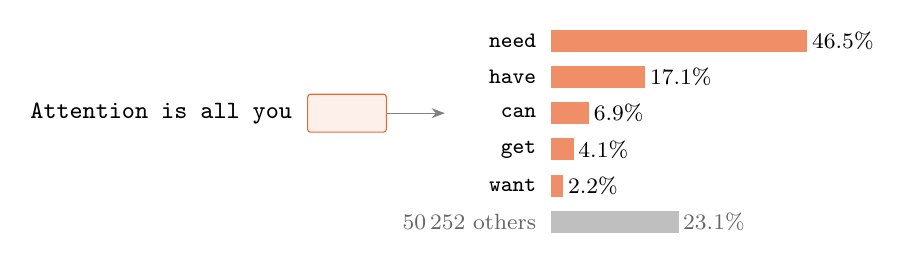
\begin{tikzpicture}[x=1mm, y=1mm, >=Stealth, font=\footnotesize]
  \node[anchor=east, font=\ttfamily\small, inner sep=1pt] (prompt) at (0,0) {Attention is all you};
  \node[draw=ctrl, fill=ctrl!10, rounded corners=1pt, minimum width=10mm, minimum height=4.8mm, anchor=west] (gap) at (1.5,0) {};
  \draw[->, black!50] (gap.east) -- (19,0);
  \foreach \tok/\p [count=\k from 0] in {need/46.5, have/17.1, can/6.9, get/4.1, want/2.2} {
    \node[anchor=east, font=\ttfamily\footnotesize, inner sep=1pt] at (31,{9.2-4.6*\k}) {\tok};
    \fill[ctrl!75] (32.5,{9.2-4.6*\k-1.4}) rectangle ++({0.7*\p},2.8);
    \node[anchor=west, inner sep=1.5pt] at ({32.5+0.7*\p},{9.2-4.6*\k}) {$\p\%$};
  }
  \node[anchor=east, inner sep=1pt, text=black!60] at (31,-13.8) {$50\,252$ others};
  \fill[black!25] (32.5,-15.2) rectangle ++({0.7*23.1},2.8);
  \node[anchor=west, inner sep=1.5pt, text=black!60] at ({32.5+0.7*23.1},-13.8) {$23.1\%$};
\end{tikzpicture}

\raggedright
\medskip
To write: \alert{sample} a token, append it, repeat.\quad {\footnotesize (GPT-2 \citep{radford2019}.)}
\takeaway{Everything today serves one function: text so far $\mapsto$ probabilities of the next token.}
\end{frame}


% =========================================================================
\begin{frame}{The whole model on one slide}
\centering
\resizebox{\linewidth}{!}{\pipeline{}{}{}{}{}}

\bigskip
\small
\renewcommand{\arraystretch}{1.5}
\begin{tabularx}{\textwidth}{@{}l l >{\raggedright\arraybackslash}X@{}}
\toprule
\alert{tokenizer} & text $\mapsto i_1,\dots,i_n\in\Vocab$ & cut the text into pieces from a fixed list \\
\alert{embedding} & $x_t=e_{i_t}+p_t\in\R^d$ & a learned vector per token, plus its position \\
\alert{attention} & $x_t\leftarrow x_t+\sum_s\alpha_{ts}\,v_s$ & the tokens exchange information \\
\alert{MLP} & $x_t\leftarrow x_t+\MLP(x_t)$ & each token is processed on its own \\
\alert{read-out} & $\softmax(Wx_n)\in\R^{|\Vocab|}$ & a probability for every token of $\Vocab$ \\
\bottomrule
\end{tabularx}

\medskip
\raggedright
Attention and MLP are repeated $L$ times. We go through the picture from left to right.
\end{frame}


% #########################################################################
% 1. WHY ATTENTION?
% #########################################################################

\section{Why attention? A short history}

% =========================================================================
% The sample is Shannon's "second-order word approximation" (1948, section 3), verbatim.
\begin{frame}{Language models before attention}
\small
\begin{mathbox}{C.~Shannon, 1948 \citep{shannon1948}: each word drawn given the one before, from counts}
\ttfamily\footnotesize THE HEAD AND IN FRONTAL ATTACK ON AN ENGLISH WRITER THAT THE CHARACTER OF THIS POINT IS THEREFORE ANOTHER METHOD FOR THE LETTERS THAT THE TIME OF WHO EVER TOLD THE PROBLEM FOR AN UNEXPECTED
\end{mathbox}

\bigskip
\centering
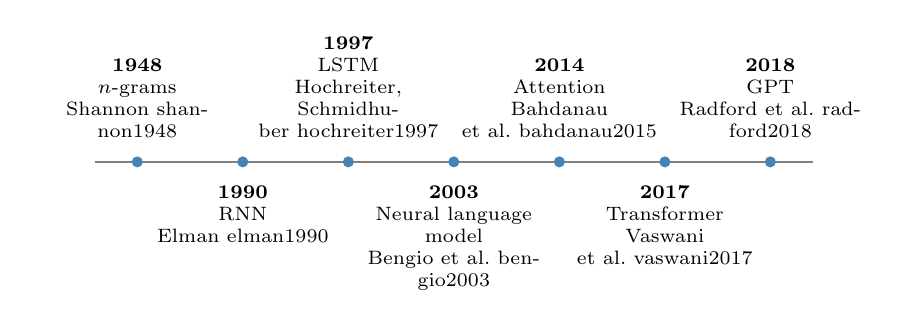
\begin{tikzpicture}[x=1.34cm, y=1cm, every node/.style={font=\scriptsize}]
  \draw[gray, line width=0.8pt] (-0.4,0) -- (6.4,0);
  \foreach \x/\yr/\txt/\anc/\dy in {
     0/1948/{\alert{$n$-grams}\\Shannon~\citep{shannon1948}}/south/0.18,
     1/1990/{\alert{RNN}\\Elman~\citep{elman1990}}/north/-0.18,
     2/1997/{\alert{LSTM}\\Hochreiter, Schmidhuber~\citep{hochreiter1997}}/south/0.18,
     3/2003/{\alert{Neural language}\\\alert{model}\\Bengio et~al.~\citep{bengio2003}}/north/-0.18,
     4/2014/{\alert{Attention}\\Bahdanau et~al.~\citep{bahdanau2015}}/south/0.18,
     5/2017/{\alert{Transformer}\\Vaswani et~al.~\citep{vaswani2017}}/north/-0.18,
     6/2018/{\alert{GPT}\\Radford et~al.~\citep{radford2018}}/south/0.18}
  {
    \fill[boxframe] (\x,0) circle (2pt);
    \node[anchor=\anc, align=center, text width=2.55cm] at (\x,\dy) {\textbf{\yr}\\\txt};
  }
\end{tikzpicture}

\bigskip
\raggedright
\takeaway{From 1990 to 2017 the model of a text is \alert{recurrent}: it reads one token at a time.}
\end{frame}


% =========================================================================
% Figure: figures/part0_recurrent.py (recurrent_panels.pdf), as in the frame "Recurrent networks read
% one token at a time" of self_attention_and_transformers.tex.  Left: |d y_n / d x_t| at
% initialization, n = 100; right: "recall the first token" (one of 8 symbols, then n - 1 fillers;
% chance 12.5%), accuracy after training with the same budget for the three models.
\begin{frame}{A recurrent network reads one token at a time}
\small
\begin{columns}[c]
\begin{column}{0.42\textwidth}
\centering
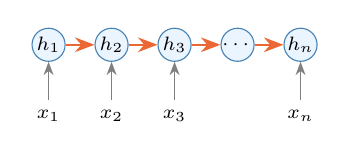
\begin{tikzpicture}[x=8mm, y=1mm, >=Stealth, font=\scriptsize,
    tok/.style={circle, draw=boxframe, fill=boxbg, inner sep=0pt, minimum size=4.2mm}]
  \foreach \i/\l in {1/h_1,2/h_2,3/h_3,4/\cdots,5/h_n} \node[tok] (h\i) at (\i,0) {$\l$};
  \foreach \i [evaluate=\i as \j using int(\i+1)] in {1,...,4} \draw[->, ctrl, line width=0.9pt] (h\i) -- (h\j);
  \foreach \i/\l in {1/x_1,2/x_2,3/x_3,5/x_n} {\node (x\i) at (\i,-9) {$\l$}; \draw[->, black!50] (x\i) -- (h\i);}
\end{tikzpicture}

\smallskip
$h_t=\tanh(W\,h_{t-1}+U\,x_t)$
\end{column}
\begin{column}{0.56\textwidth}
\footnotesize
\begin{enumerate}
\item \alert{Sequential}: $h_t$ needs $h_{t-1}$; the $n$ steps cannot run in parallel.
\item \alert{Fading memory}: $x_1$ reaches $h_n$ through $n-1$ multiplications, so its influence and its gradient shrink geometrically \citep{bengio1994}.
\end{enumerate}
The LSTM \citep{hochreiter1997} adds a gated memory: it helps, it does not cure.
\end{column}
\end{columns}

\smallskip
\centering
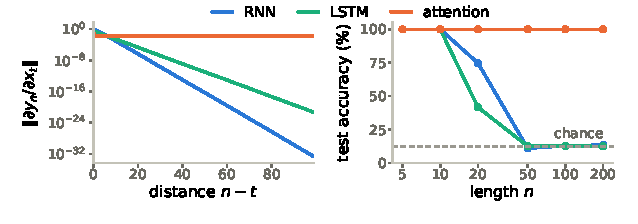
\includegraphics[width=0.86\linewidth]{recurrent_panels.pdf}

{\raggedright\scriptsize Left: influence of token $t$ on the output at $n=100$. Right: the task ``repeat the first token'', after training.\par}
\takeaway{The longer the text, the harder it is to remember its beginning.}
\end{frame}


% =========================================================================
% Table 1 of Vaswani et al. (2017), recurrent and self-attention rows only.
\begin{frame}{Attention: every token is one step from every other}
\small
\tikzset{
  tok/.style={circle, draw=boxframe, fill=boxbg, inner sep=0pt, minimum size=2.6mm},
  edge/.style={black!35, line width=0.4pt},
  hot/.style={ctrl, line width=0.9pt},
}
\begin{columns}[T]
\begin{column}{0.5\textwidth}
\centering
\alert{Recurrent}\\[1pt]
\begin{tikzpicture}[x=7.5mm, y=1mm, >=Stealth, font=\scriptsize]
  \foreach \i in {1,...,6} \node[tok] (r\i) at (\i,0) {};
  \foreach \i [evaluate=\i as \j using int(\i+1)] in {1,...,5} \draw[->, hot] (r\i) -- (r\j);
  \node[below=0.5mm] at (r1.south) {$x_1$};
  \node[below=0.5mm] at (r6.south) {$x_n$};
  \node[above, text=ctrl, inner sep=1pt] at (3.5,1.6) {$n-1$ steps from $x_1$ to $x_n$};
\end{tikzpicture}
\end{column}
\begin{column}{0.5\textwidth}
\centering
\alert{Self-attention}\\[1pt]
\begin{tikzpicture}[x=7.5mm, y=1mm, >=Stealth, font=\scriptsize]
  \foreach \i in {1,...,6} \node[tok] (a\i) at (\i,0) {};
  \foreach \i in {1,...,5} \foreach \j in {\i,...,6}
    {\ifnum\i<\j \draw[edge] (a\i.north) .. controls +({0.12*(\j-\i)},{1.2*(\j-\i)}) and +({-0.12*(\j-\i)},{1.2*(\j-\i)}) .. (a\j.north);\fi}
  \draw[hot] (a1.north) .. controls +(0.6,6) and +(-0.6,6) .. (a6.north);
  \node[below=0.5mm] at (a1.south) {$x_1$};
  \node[below=0.5mm] at (a6.south) {$x_n$};
  \node[above, text=ctrl, inner sep=1pt] at (3.5,5.8) {$1$ step from $x_1$ to $x_n$};
\end{tikzpicture}
\end{column}
\end{columns}

\bigskip
\centering
\renewcommand{\arraystretch}{1.15}
\begin{tabular}{@{}l c c c@{}}
\toprule
 & \textbf{Operations} & \textbf{Sequential steps} & \textbf{Longest path} \\
\midrule
Recurrent & $O(n\,d^2)$ & $O(n)$ & $O(n)$ \\
Self-attention & $O(n^2d)$ & \alert{$O(1)$} & \alert{$O(1)$} \\
\bottomrule
\end{tabular}

\smallskip
{\footnotesize Per layer, $n$ tokens of width $d$: Table~1 of \citet{vaswani2017}.\par}
\takeaway{Attention does more operations, but all at once, and any two tokens are one step apart.}
\end{frame}


% =========================================================================
% A schematic, not a measurement: the lines from "Hund" are drawn with made-up opacities.
\begin{frame}{2014: attention is born in machine translation}
\small
A recurrent translator squeezed the whole input sentence into its last state $h_n$. Bahdanau, Cho and Bengio \citep{bahdanau2015}: let every output word \alert{look back} at all the input states,
\[
c_t=\sum_{s=1}^n\alpha_{ts}\,h_s,\qquad \alpha_{ts}=\softmax_s\big(\score(q_t,h_s)\big),\qquad \textstyle\sum_s\alpha_{ts}=1.
\]

\centering
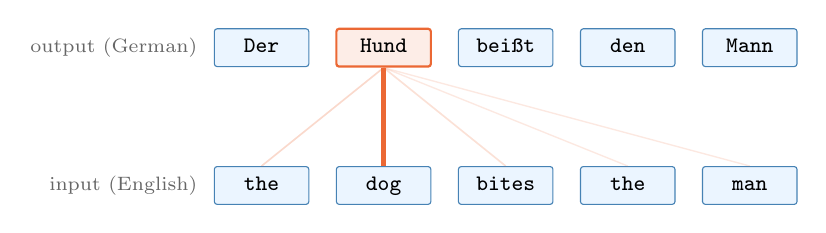
\begin{tikzpicture}[x=1.55cm, y=1cm, >=Stealth, font=\footnotesize,
    w/.style={draw=boxframe, fill=boxbg, rounded corners=1pt, minimum height=4.8mm, minimum width=12mm,
              inner sep=1pt, font=\ttfamily\footnotesize},
    lab/.style={anchor=east, inner sep=1pt, text=black!60, font=\scriptsize}]
  \foreach \t/\w in {0/the, 1/dog, 2/bites, 3/the, 4/man} \node[w] (s\t) at (\t,0) {\strut\w};
  \foreach \t/\w in {0/Der, 2/beißt, 3/den, 4/Mann} \node[w] (o\t) at (\t,1.75) {\strut\w};
  \node[w, draw=ctrl, fill=ctrl!12, line width=0.8pt] (o1) at (1,1.75) {\strut Hund};
  \foreach \t/\op/\lw in {0/0.25/0.6, 1/1/1.8, 2/0.2/0.6, 3/0.15/0.5, 4/0.15/0.5}
    \draw[ctrl, line width=\lw pt, opacity=\op] (o1.south) -- (s\t.north);
  \node[lab] at (-0.5,0) {input (English)};
  \node[lab] at (-0.5,1.75) {output (German)};
\end{tikzpicture}

\raggedright
{\footnotesize Schematic: when writing \texttt{Hund}, the weights $\alpha_{ts}$ concentrate on \texttt{dog}. Nobody labels this alignment: it is learned.\par}
\takeaway{Attention = a learned, soft alignment between the words.}
\end{frame}


% =========================================================================
% The table of L. Weng's post "Attention? Attention!" (2018), in the notation of this lecture, as in
% the frame "Attention before 2017: a table of scores" of self_attention_and_transformers.tex.
\begin{frame}{Attention before 2017: a table of scores}
\small
How should the query $q$ be compared with a key $k$? Several answers, 2014--2017:

\medskip
\footnotesize
{\centering
\renewcommand{\arraystretch}{1.2}
\begin{tabular}{@{}l l l@{}}
\toprule
\textbf{Name} & \textbf{$\score(q,k)$} & \textbf{Table of L.~Weng \citep{weng2018}} \\
\midrule
content-based & $\cos(q,k)$ & Graves et~al., 2014 \citep{graves2014} \\
additive & $v^\top\tanh\big(W[q;k]\big)$ & Bahdanau et~al., 2015 \citep{bahdanau2015} \\
location-based & $Wq$\quad (no key) & Luong et~al., 2015 \citep{luong2015} \\
general & $q^\top Wk$ & Luong et~al., 2015 \citep{luong2015} \\
dot product & $q^\top k$ & Luong et~al., 2015 \citep{luong2015} \\
\rowcolor{ctrl!12}\alert{scaled dot product} & $q^\top k/\sqrt d$ & Vaswani et~al., 2017 \citep{vaswani2017} \\
\bottomrule
\end{tabular}\par}

\medskip
\small
\alert{2017.} The score is almost not new: $q^\top k/\sqrt d$ is the dot product, rescaled (why, in section 3). New is what was \alert{removed}: the recurrent network. Hence the title, \emph{Attention is all you need}.
\takeaway{The transformer keeps the attention of 2014 and throws away the recurrence.}
\end{frame}


% #########################################################################
% 2. FROM TEXT TO VECTORS
% #########################################################################

\section{From text to vectors}

% =========================================================================
% The examples are those of self_attention_and_transformers.tex: the byte-pair encoding learned on
% Shakespeare (figures/part1_tokenizer.py) splits " Erlangen" (never in the text) into
% Er|l|ang|en and keeps " gentleman" (77 times) whole, after 10 000 merges; GPT-2 has 50 257 tokens
% and 1.15 tokens per English word on the Universal Declaration of Human Rights.
\begin{frame}{Tokens: characters, words, or something in between?}
\small
The network reads \alert{integers}: first we must cut the text into pieces from a fixed list $\Vocab$.

\medskip
\footnotesize
\renewcommand{\arraystretch}{1.4}
\begin{tabularx}{\textwidth}{@{}l l >{\raggedright\arraybackslash}X@{}}
\toprule
\textbf{Pieces} & \textbf{Size of $\Vocab$} & \textbf{Problem} \\
\midrule
characters & $\approx100$ & long sequences: one token per letter, and the cost of attention grows like $n^2$ \\
words & huge, never complete & a word never seen (\texttt{Erlangen}, a typo, a new name) has no token \\
\rowcolor{ctrl!12}\alert{subwords} & $50\,257$ in GPT-2 & frequent words whole, rare words in pieces: \texttt{Er|l|ang|en} \\
\bottomrule
\end{tabularx}

\medskip
\small
Subwords are the compromise: about $1.15$ tokens per English word, and \alert{every} text can be written, since the single bytes are tokens too.
\takeaway{A tokenizer trades the size of the vocabulary against the length of the sequence.}
\end{frame}


% =========================================================================
% The example of Sennrich et al. (2016, section 3.2): {low: 5, lower: 2, newest: 6, widest: 3}.  The
% counts were checked by running the algorithm: merge 1 is a tie, e+s and s+t both 9; merge 3 is a
% tie, l+o and o+w both 7 (the first is taken).
\begin{frame}{Byte-pair encoding: merge the most frequent pair}
\small
Start from single characters. Repeat: count the neighbouring pairs, \alert{merge the most frequent one} into a new token \citep{gage1994,sennrich2016}.

\medskip
\footnotesize
Corpus: \texttt{low}\,$\times5$,\ \ \texttt{lower}\,$\times2$,\ \ \texttt{newest}\,$\times6$,\ \ \texttt{widest}\,$\times3$.

\smallskip
\def\b{\textcolor{black!40}{|}}
\renewcommand{\arraystretch}{1.25}
\begin{tabularx}{\textwidth}{@{}c l c >{\ttfamily\raggedright\arraybackslash}X@{}}
\toprule
\textbf{merge} & \textbf{pair} & \textbf{count} & \normalfont\textbf{the words after the merge} \\
\midrule
0 & & & l\b o\b w \quad l\b o\b w\b e\b r \quad n\b e\b w\b e\b s\b t \quad w\b i\b d\b e\b s\b t \\
1 & \texttt{e}\,+\,\texttt{s} & 9 & l\b o\b w \quad l\b o\b w\b e\b r \quad n\b e\b w\b \alert{es}\b t \quad w\b i\b d\b \alert{es}\b t \\
2 & \texttt{es}\,+\,\texttt{t} & 9 & l\b o\b w \quad l\b o\b w\b e\b r \quad n\b e\b w\b \alert{est} \quad w\b i\b d\b \alert{est} \\
3 & \texttt{l}\,+\,\texttt{o} & 7 & \leavevmode\alert{lo}\b w \quad \alert{lo}\b w\b e\b r \quad n\b e\b w\b est \quad w\b i\b d\b est \\
4 & \texttt{lo}\,+\,\texttt{w} & 7 & \leavevmode\alert{low} \quad \alert{low}\b e\b r \quad n\b e\b w\b est \quad w\b i\b d\b est \\
\bottomrule
\end{tabularx}

\medskip
\small
A word never seen: \texttt{lowest} $\to$ \texttt{low\b est}. GPT-2: the same, $50\,000$ merges on the bytes of web text \citep{radford2019}.
\takeaway{Frequent words become one token; rare words are spelled with frequent pieces.}
\end{frame}


% =========================================================================
% figures/part1_tokenizer.py prints every example and draws tokens_udhr.pdf, as in the frame "The
% tokens of GPT-2 are neither words nor letters" of self_attention_and_transformers.tex.
\begin{frame}{The tokens of GPT-2 are neither words nor letters}
\def\b{\textcolor{black!40}{|}}
\centering
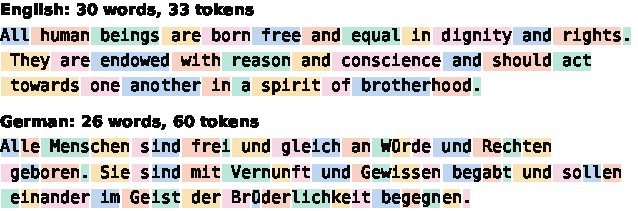
\includegraphics{tokens_udhr.pdf}

\medskip
\scriptsize
\renewcommand{\arraystretch}{1.15}
\begin{tabularx}{\textwidth}{@{}l X@{}}
\toprule
letters & \texttt{strawberry} $\to$ \texttt{st\b raw\b berry};\quad \texttt{\textvisiblespace strawberry} $\to$ one token: how many r? \\
capitals, spaces & \texttt{the}, \texttt{\textvisiblespace the}, \texttt{The}, \texttt{\textvisiblespace The}: four unrelated tokens \\
numbers & \texttt{\textvisiblespace 1234567} $\to$ \texttt{\textvisiblespace 123\b 45\b 67} \\
German & \texttt{\textvisiblespace Prüfungsordnung} $\to$ \texttt{\textvisiblespace Pr\b ü\b f\b ung\b s\b ord\b n\b ung} \\
\bottomrule
\end{tabularx}

\medskip
\raggedright\small
All 30 articles: \alert{1.15} tokens per English word, \alert{2.82} per German word.
\takeaway{The model never sees letters, only token numbers. This explains some odd failures.}
\end{frame}


% =========================================================================
% The entries of e_{i_t} are drawn as random numbers in [-1, 1] from a fixed seed; the token
% indices are those of the tokenizer of GPT-2 (figures/gpt2.py).
\begin{frame}{Embedding: one learned vector per token}
\begin{columns}[c]
\begin{column}{0.57\textwidth}
\centering
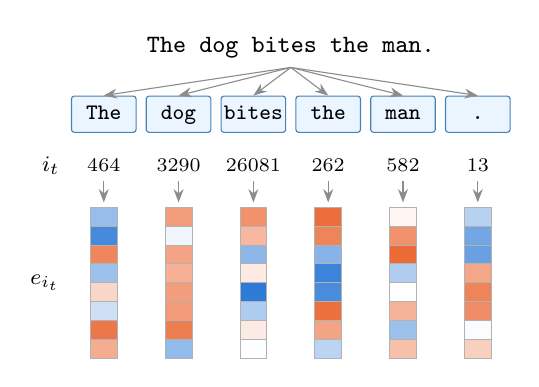
\begin{tikzpicture}[x=0.95cm, y=1cm, >=Stealth, font=\footnotesize,
    tok/.style={draw=boxframe, fill=boxbg, rounded corners=1pt, minimum height=4.6mm, minimum width=8.2mm,
                inner sep=1pt, font=\ttfamily\footnotesize},
    cell/.style={minimum width=3.4mm, minimum height=2.4mm, inner sep=0pt, line width=0.3pt},
    lab/.style={anchor=east, inner sep=1pt}]
  \node[font=\ttfamily\small] (text) at (2.5,0) {The dog bites the man.};
  \pgfmathsetseed{2026}
  \foreach \t/\w/\i in {0/The/464, 1/dog/3290, 2/bites/26081, 3/the/262, 4/man/582, 5/./13} {
    \node[tok] (t\t) at (\t,-0.85) {\strut\w};
    \draw[->, black!45] (text.south) -- (t\t.north);
    \node[font=\scriptsize] (i\t) at (\t,-1.5) {\i};
    \draw[->, black!45] (i\t.south) -- (\t,-1.97);
    \foreach \k in {0,...,7} {
      \pgfmathsetmacro\v{rand}
      \pgfmathtruncatemacro\pct{round(100*abs(\v))}
      \pgfmathtruncatemacro\isneg{\v<0}
      \ifnum\isneg=1 \def\pc{posneg}\else\def\pc{ctrl}\fi
      \node[cell, draw=black!30, fill=\pc!\pct!white] at (\t,-2.15-0.24*\k) {};
    }
  }
  \node[lab] at (-0.55,-1.5) {$i_t$};
  \node[lab] at (-0.55,-2.99) {$e_{i_t}$};
\end{tikzpicture}
\end{column}
\begin{column}{0.41\textwidth}
\small
A table $E\in\R^{|\Vocab|\times d}$ with one row per token:
\[
x_t=e_{i_t}=E^\top\mathbf 1_{i_t}\in\R^d .
\]
A look-up is a linear map applied to a one-hot vector $\mathbf 1_{i_t}$, so $E$ is \alert{learned by gradient descent} with everything else.

\medskip
\scriptsize
Drawn: $d=8$. GPT-2: $|\Vocab|=50\,257$, $d=768$, that is $38.6$ million numbers.
\end{column}
\end{columns}
\takeaway{Token number $\mapsto$ vector: the first layer of the network is a table.}
\end{frame}


% =========================================================================
% figures/part1_embeddings.py: nearest rows of the token embedding of GPT-2 in cosine similarity,
% nothing filtered, as in the frame "Similar tokens, similar vectors" of
% self_attention_and_transformers.tex.
\begin{frame}{Similar tokens get similar vectors}
\small
In GPT-2, after training, the nearest vectors $e_j$ to some $e_i$:

\medskip
\scriptsize
\renewcommand{\arraystretch}{1.3}
\setlength{\tabcolsep}{3pt}
\begin{tabular*}{\textwidth}{@{}l@{\extracolsep{\fill}}llll@{}}
\toprule
token $i$ & \multicolumn{4}{l}{nearest tokens $j$, by $\cos(e_i,e_j)$} \\
\midrule
\texttt{\textvisiblespace Germany}     & \texttt{Germany} .86      & \texttt{\textvisiblespace German} .75     & \texttt{German} .71        & \texttt{\textvisiblespace France} .70 \\
\texttt{\textvisiblespace mathematics} & \texttt{\textvisiblespace Mathematics} .82 & \texttt{\textvisiblespace mathematical} .78 & \texttt{\textvisiblespace maths} .76 & \texttt{\textvisiblespace math} .75 \\
\texttt{\textvisiblespace Monday}      & \texttt{\textvisiblespace Tuesday} .89  & \texttt{\textvisiblespace Thursday} .85   & \texttt{\textvisiblespace Wednesday} .84 & \texttt{\textvisiblespace Friday} .82 \\
\texttt{\textvisiblespace seven}       & \texttt{\textvisiblespace six} .87      & \texttt{\textvisiblespace eight} .86      & \texttt{\textvisiblespace five} .85      & \texttt{\textvisiblespace nine} .85 \\
\texttt{\textvisiblespace river}       & \texttt{\textvisiblespace rivers} .78   & \texttt{\textvisiblespace River} .74      & \texttt{\textvisiblespace lake} .66      & \texttt{\textvisiblespace creek} .64 \\
\bottomrule
\end{tabular*}

\medskip
\small
Two random tokens: $\cos(e_i,e_j)=0.27$ on average.
\takeaway{Nobody told the model that Monday and Tuesday belong together: predicting the next token taught it.}
\end{frame}


% #########################################################################
% 3. SELF-ATTENTION
% #########################################################################

\section{Self-attention}

% =========================================================================
% Figure: figures/part2_attention.py, section 1 (lookup_weights.pdf): a query at 50 degrees and eight
% keys on the unit circle; the largest weight is 0.27, 0.59 and 0.97 for beta = 1, 4, 16.
\begin{frame}{Attention is a soft look-up table}
\small
A Python dictionary: keys $k_s$, values $v_s$. A query $q$ returns the value of the key that \alert{equals} $q$.

Attention: return a \alert{weighted average} of all the values, with more weight on keys similar to $q$:
\[
\text{out}=\sum_s\alpha_s\,v_s,\qquad \alpha_s=\softmax_s\big(\ctrl{\beta}\,\langle q,k_s\rangle\big)=\frac{e^{\beta\langle q,k_s\rangle}}{\sum_r e^{\beta\langle q,k_r\rangle}} .
\]

\centering
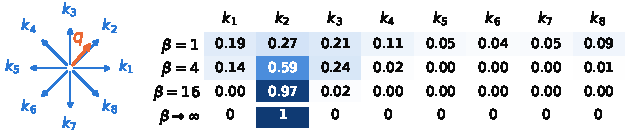
\includegraphics{lookup_weights.pdf}

\raggedright
{\scriptsize One query, eight keys on the unit circle. $\ctrl{\beta}\to\infty$: all the weight on the nearest key, a look-up. (With a fixed kernel: the regression of Nadaraya and Watson, 1964 \citep{nadaraya1964,watson1964}.)\par}

\smallskip
For finite $\beta$ the output is differentiable in $q$, $k_s$, $v_s$: \alert{the table can be learned}.
\takeaway{Attention = a dictionary look-up made smooth, hence trainable.}
\end{frame}


% =========================================================================
\begin{frame}[fragile]{Self-attention: every token asks, every token answers}
\small
The tokens $x_1,\dots,x_n\in\R^d$ are the rows of $X$. Three learned matrices make three versions of each token:

\medskip
\footnotesize
\renewcommand{\arraystretch}{1.2}
\begin{tabular}{@{}l l l@{}}
\alert{query} & $Q=XW_Q$ & what token $t$ is looking for \\
\alert{key}   & $K=XW_K$ & what token $s$ offers \\
\alert{value} & $V=XW_V$ & what token $s$ passes on \\
\end{tabular}

\small
\[
\ctrl{\alpha_{ts}}=\softmax_s\Big(\frac{\langle q_t,k_s\rangle}{\sqrt{d_a}}\Big),\qquad
y_t=\sum_{s=1}^n\ctrl{\alpha_{ts}}\,v_s
\quad\Longleftrightarrow\quad
Y=\softmax\Big(\frac{QK^\top}{\sqrt{d_a}}\Big)V .
\]
\begin{lstlisting}
def attention(X, Wq, Wk, Wv):
    Q, K, V = X @ Wq, X @ Wk, X @ Wv                # one row per token
    A = (Q @ K.T / K.shape[-1] ** 0.5).softmax(-1)  # (n, n), rows sum to 1
    return A @ V                                    # weighted means of values
\end{lstlisting}
\footnotesize $d_a$: the length of a query and of a key. Each row of $A=(\alpha_{ts})$ is a probability vector.
\takeaway{Learned: only $W_Q,W_K,W_V$. Who looks at whom is decided by the input itself.}
\end{frame}


% =========================================================================
% figures/part2_gpt2_attention.py (gpt2_attention_one.pdf): the sentence of Wang et al. (2023), with
% <|endoftext|> first; head 9 of block 9 (counted from 0).
\begin{frame}{In a trained model: who looks at whom}
\small
GPT-2 reads \texttt{When Mary and John went to the store, John gave a drink to} \dots

\medskip
\centering
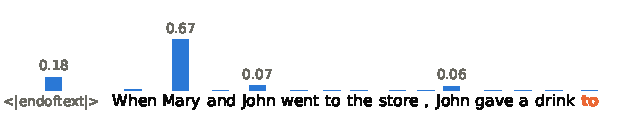
\includegraphics{gpt2_attention_one.pdf}

\raggedright
\footnotesize
One head of GPT-2 \citep{wang2023}: the weights $\ctrl{\alpha_{ns}}$ of the last token \texttt{to} over all earlier tokens.

\medskip
\small
It looks at \texttt{Mary}, and the model predicts \texttt{Mary} with probability $0.68$, \texttt{John} with $0.02$.
\takeaway{Heads learn jobs. This one: find the name that has not been used yet.}
\end{frame}


% =========================================================================
% figures/part2_gpt2_attention.py (gpt2_attention_heads.pdf).
\begin{frame}{Multi-head attention: several look-ups in parallel}
\small
One softmax gives one notion of ``relevant''. Use $H$ heads, each with its own $W_Q^h,W_K^h,W_V^h$ of width $d/H$, and glue the results:
\[
\text{MHA}(X)=\big[\,Y^1\ \big|\ Y^2\ \big|\ \cdots\ \big|\ Y^H\,\big]\,W_O,\qquad
Y^h=\softmax\Big(\frac{Q^hK^{h\top}}{\sqrt{d/H}}\Big)V^h .
\]
About the same cost as one head of width $d$. GPT-2: $12$ heads of width $64$ in each of $12$ blocks.

\centering
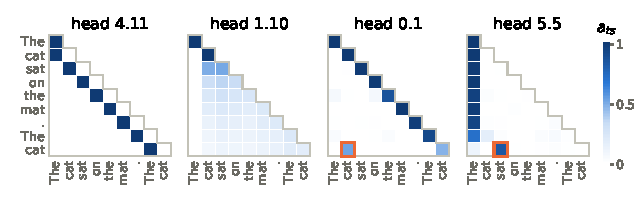
\includegraphics[width=0.9\linewidth]{gpt2_attention_heads.pdf}

\raggedright\scriptsize
Four of its 144 heads: the previous token; all tokens so far, alike; the same token; the token after the earlier \texttt{cat}.
\takeaway{Different heads, different questions, computed at the same time.}
\end{frame}


% =========================================================================
% Figure: figures/part2_attention.py, section 2 (scaling_softmax.pdf): n = 64 queries and keys with
% independent N(0, 1) entries, 200 draws for each d.  softmax(1, 2, 3) = (0.090, 0.245, 0.665);
% softmax(10, 20, 30) = (2.1e-9, 4.5e-5, 0.99995).
\begin{frame}{Why divide by $\sqrt{d_a}$?}
\small
\alert{1. Large scores freeze the softmax.}
\[
\softmax(1,2,3)=(0.09,\ 0.24,\ 0.67),\qquad
\softmax(10,20,30)\approx(0,\ 0,\ 1).
\]
A one-hot output barely moves when the scores move: its derivative $\operatorname{diag}(\alpha)-\alpha\alpha^\top\approx0$, so \alert{$W_Q$ and $W_K$ stop learning}.

\bigskip
\alert{2. Scores grow with the width.} If $q,k\in\R^{d_a}$ have independent entries of mean $0$ and variance $1$,
\[
\E\langle q,k\rangle=\sum_{j=1}^{d_a}\E q_j\,\E k_j=0,\qquad
\Var\langle q,k\rangle=\sum_{j=1}^{d_a}\E q_j^2\,\E k_j^2=d_a .
\]
So $\langle q,k\rangle$ is typically of size $\sqrt{d_a}$: $\sqrt{64}=8$ for a head of GPT-2.

\bigskip
\alert{The fix:} divide by $\sqrt{d_a}$. Then $\langle q,k\rangle/\sqrt{d_a}$ has variance $1$ at \emph{every} width.
\takeaway{Dividing by $\sqrt{d_a}$ keeps the softmax soft, so gradients reach $W_Q$ and $W_K$.}
\end{frame}


% =========================================================================
% figures/part2_attention.py, section 2: at d = 1024 the largest weight of a row is 0.947 on average
% without the factor and 0.107 with it; the median Frobenius norm of the Jacobian of the softmax is
% 2.8e-4 without and 0.18 with it (ratio 640).
\begin{frame}{The $\sqrt{d_a}$, measured}
\small
$n=64$ queries and keys with independent $N(0,1)$ entries, drawn $200$ times for each width $d$:

\medskip
\centering
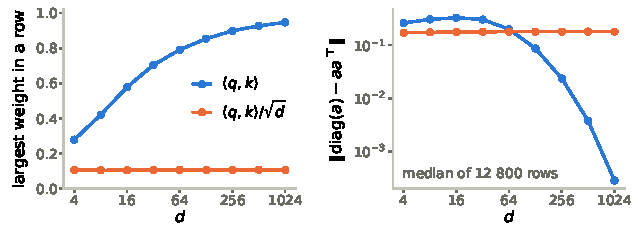
\includegraphics{scaling_softmax.pdf}

\medskip
\raggedright
\footnotesize
Left: the largest weight of a row; $1/64$ would be uniform, $1$ a look-up.\quad Right: the size of the derivative of the softmax.

\medskip
\small
Without the factor, at $d=1024$ the largest weight is $0.95$ on average (with it, $0.11$), and the derivative is about $600$ times smaller.
\takeaway{Without $\sqrt{d_a}$, the wider the model, the less its attention can learn.}
\end{frame}


% #########################################################################
% 4. WORD ORDER
% #########################################################################

\section{Word order: positions and masks}

% =========================================================================
% The four panels: figures/part2_attention.py, section 3 (six tokens in R^8, f(x) = x +
% attention(x) for nn.MultiheadAttention(8, 2), the permutation (1, 4, 2, 6, 3, 5)).
\tikzset{
  cdsquare/.style={x=1mm, y=1mm, >=Stealth, font=\footnotesize},
  cdcorner/.style={inner sep=0pt},
  cdlabel/.style={font=\footnotesize, inner sep=1.5pt, text height=1.7ex, text depth=0.5ex},
}
\begin{frame}{Attention does not see the order}
\small
\begin{mathbox}{Proposition (permutation equivariance)}
Let $f(x)_t=x_t+\sum_s\alpha_{ts}(x)\,v_s$ and $(Px)_t=x_{\pi(t)}$ for a permutation $\pi$ of the tokens. Then $f(Px)=P\,f(x)$.
\end{mathbox}

\smallskip
\begin{columns}[c]
\begin{column}{0.45\textwidth}
\centering
\scalebox{0.85}{\begin{tikzpicture}[cdsquare]
  \node[cdcorner] (x)   at (0,0)    {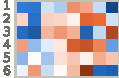
\includegraphics{equivariance_x.pdf}};
  \node[cdcorner] (fx)  at (29,0)   {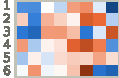
\includegraphics{equivariance_fx.pdf}};
  \node[cdcorner] (Px)  at (0,-25)  {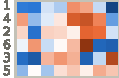
\includegraphics{equivariance_Px.pdf}};
  \node[cdcorner] (fPx) at (29,-25) {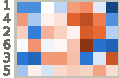
\includegraphics{equivariance_fPx.pdf}};
  \draw[->] ([xshift=1mm]x.east)  -- node[above] {$f$} ([xshift=-1mm]fx.west);
  \draw[->] ([xshift=1mm]Px.east) -- node[below] {$f$} ([xshift=-1mm]fPx.west);
  \draw[->] ([yshift=-1mm]x.south)  -- node[left]  {$P$} ([yshift=1mm]Px.north);
  \draw[->] ([yshift=-1mm]fx.south) -- node[right] {$P$} ([yshift=1mm]fPx.north);
  \node[cdlabel, above] at (x.north)   {$x$};
  \node[cdlabel, above] at (fx.north)  {$f(x)$};
  \node[cdlabel, below] at (Px.south)  {$Px$};
  \node[cdlabel, below] at (fPx.south) {$f(Px)=P\,f(x)$};
\end{tikzpicture}}
\end{column}
\begin{column}{0.53\textwidth}
\footnotesize
\texttt{The dog bites the man.}\\\texttt{The man bites the dog.}\\
Same tokens, so the same vectors, in another order.

\medskip
\emph{Why.} $\alpha_{ts}$ depends only on the pair $(x_t,x_s)$ and on a sum over \emph{all} tokens; a sum does not care about the order of its terms.

\medskip
The MLP and the normalization act on each token separately: the whole transformer is equivariant.
\end{column}
\end{columns}
\takeaway{Without help, a transformer reads a \alert{bag of tokens}.}
\end{frame}


% =========================================================================
% The values of p_t (d = 8, t = 0..5) are computed below with the formula on the right; the entries
% of e_{i_t} are the random numbers of the embedding frame (the same seed).
\begin{frame}{Positional encoding: tell each token where it is}
\begin{columns}[c]
\begin{column}{0.57\textwidth}
\centering
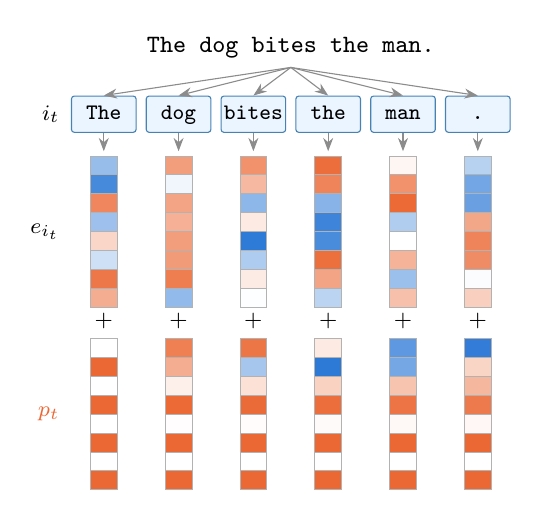
\begin{tikzpicture}[x=0.95cm, y=1cm, >=Stealth, font=\footnotesize,
    tok/.style={draw=boxframe, fill=boxbg, rounded corners=1pt, minimum height=4.6mm, minimum width=8.2mm,
                inner sep=1pt, font=\ttfamily\footnotesize},
    cell/.style={minimum width=3.4mm, minimum height=2.4mm, inner sep=0pt, line width=0.3pt},
    lab/.style={anchor=east, inner sep=1pt}]
  \node[font=\ttfamily\small] (text) at (2.5,0) {The dog bites the man.};
  \pgfmathsetseed{2026}
  \foreach \t/\w in {0/The, 1/dog, 2/bites, 3/the, 4/man, 5/.} {
    \node[tok] (t\t) at (\t,-0.85) {\strut\w};
    \draw[->, black!45] (text.south) -- (t\t.north);
    \draw[->, black!45] (t\t.south) -- (\t,-1.32);
    \foreach \k in {0,...,7} {
      \pgfmathsetmacro\v{rand}
      \pgfmathtruncatemacro\pct{round(100*abs(\v))}
      \pgfmathtruncatemacro\isneg{\v<0}
      \ifnum\isneg=1 \def\pc{posneg}\else\def\pc{ctrl}\fi
      \node[cell, draw=black!30, fill=\pc!\pct!white] at (\t,-1.5-0.24*\k) {};
      \pgfmathsetmacro\angle{10000^(-2*floor(\k/2)/8)*\t}
      \pgfmathsetmacro\v{mod(\k,2)==0 ? sin(\angle r) : cos(\angle r)}
      \pgfmathtruncatemacro\pct{round(100*abs(\v))}
      \pgfmathtruncatemacro\isneg{\v<0}
      \ifnum\isneg=1 \def\pc{posneg}\else\def\pc{ctrl}\fi
      \node[cell, draw=black!30, fill=\pc!\pct!white] at (\t,-3.82-0.24*\k) {};
    }
    \node at (\t,-3.47) {$+$};
  }
  \node[lab] at (-0.55,-0.85) {$i_t$};
  \node[lab] at (-0.55,-2.34) {$e_{i_t}$};
  \node[lab] at (-0.55,-4.66) {$\ctrl{p_t}$};
\end{tikzpicture}
\end{column}
\begin{column}{0.41\textwidth}
\small
Add a vector that depends only on the position $t$:
\begin{align*}
x_t&=e_{i_t}+\ctrl{p_t}\\
\ctrl{p_t}&=\big(\sin\omega_jt,\ \cos\omega_jt\big)_{j<d/2}\\
\omega_j&=10000^{-2j/d}
\end{align*}
\footnotesize
A \alert{clock with many hands}: fast ones tell neighbours apart, slow ones give the rough place in the text \citep{vaswani2017}.

\medskip
GPT-2 \emph{learns} $p_t$ instead; recent models rotate $q_t$ and $k_s$ by angles proportional to $t$ and $s$ \citep{su2024}.
\end{column}
\end{columns}
\takeaway{Now \texttt{dog} at position 2 and \texttt{dog} at position 5 are different vectors: the order is in the input.}
\end{frame}


% =========================================================================
% Figure, listing and output: figures/part2_attention.py, section 4 (six random tokens in R^16 and a
% random layer, not a trained model).
\begin{frame}[fragile]{Masking: no looking ahead}
\small
A language model predicts token $t+1$ from tokens $1,\dots,t$ only. Set the scores with $s>t$ to $-\infty$ \alert{before} the softmax: their weights become exactly $0$.

\centering
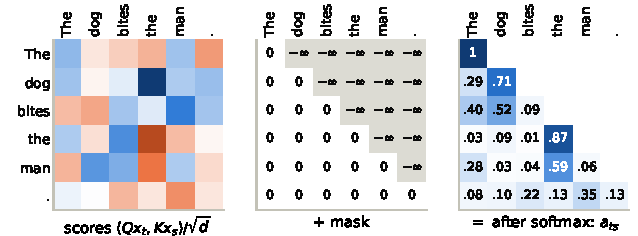
\includegraphics[width=0.9\linewidth]{mask_matrices.pdf}

{\raggedright\scriptsize A random layer on \texttt{The dog bites the man.}: scores, scores with the mask, weights $\alpha_{ts}$ (each row sums to $1$).\par}

\begin{lstlisting}
future = torch.ones(n, n).triu(1).bool()            # True where s > t
A = scores.masked_fill(future, -torch.inf).softmax(-1)
\end{lstlisting}
\takeaway{Order enters a transformer through two doors only: the positions and the mask.}
\end{frame}


% #########################################################################
% 5. THE TRANSFORMER AND ITS TRAINING
% #########################################################################

\section{The transformer and its training}

% =========================================================================
% The block of GPT-2 (pre-normalization), as in the frame "The transformer block" of
% self_attention_and_transformers.tex; the parameter count is printed by figures/gpt2.py.
\begin{frame}{The transformer block}
\centering
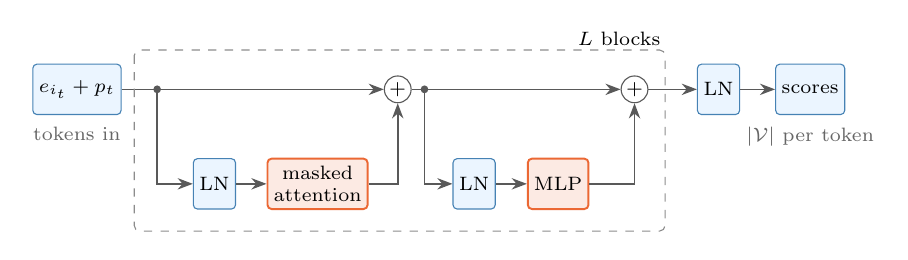
\begin{tikzpicture}[x=0.97mm, y=1mm, >=Stealth, font=\scriptsize,
    op/.style={draw=boxframe, fill=boxbg, rounded corners=1.5pt, minimum height=6.4mm, inner sep=2.2pt, align=center},
    hot/.style={draw=ctrl, fill=ctrl!14, line width=0.7pt},
    plus/.style={circle, draw=black!65, fill=white, inner sep=0pt, minimum size=3.4mm, font=\scriptsize},
    wire/.style={->, black!65, line width=0.55pt}]
  \node[op] (emb) at (7,0) {$e_{i_t}+p_t$};
  \node[plus] (p1) at (49,0) {$+$};
  \node[plus] (p2) at (80,0) {$+$};
  \node[op] (lnf) at (91,0) {LN};
  \node[op] (out) at (103,0) {scores};
  \node[op] (ln1) at (25,-12) {LN};
  \node[op, hot] (att) at (38.5,-12) {masked\\attention};
  \node[op] (ln2) at (59,-12) {LN};
  \node[op, hot] (mlp) at (70,-12) {MLP};
  \draw[wire] (emb) -- (p1);
  \draw[wire] (p1) -- (p2);
  \draw[wire] (p2) -- (lnf);
  \draw[wire] (lnf) -- (out);
  \fill[black!65] (17.5,0) circle (0.5);
  \draw[wire] (17.5,0) |- (ln1);
  \draw[wire] (ln1) -- (att);
  \draw[wire] (att) -| (p1);
  \fill[black!65] (52.5,0) circle (0.5);
  \draw[wire] (52.5,0) |- (ln2);
  \draw[wire] (ln2) -- (mlp);
  \draw[wire] (mlp) -| (p2);
  \draw[black!45, dashed, rounded corners=2pt] (14.5,5) rectangle (84,-18);
  \node[anchor=south east, inner sep=1.5pt] at (84,5) {$L$ blocks};
  \node[anchor=north, inner sep=2pt, text=black!60] at (7,-4) {tokens in};
  \node[anchor=north, inner sep=2pt, text=black!60] at (103,-4) {$|\Vocab|$ per token};
\end{tikzpicture}

\bigskip
\small
\renewcommand{\arraystretch}{1.45}
\begin{tabularx}{\textwidth}{@{}l >{\raggedright\arraybackslash}X@{}}
$x\leftarrow x+\ctrl{\Attention}(\LN(x))$ & the tokens exchange information \\
$x\leftarrow x+\ctrl{\MLP}(\LN(x))$ & each token on its own: $x_t\mapsto W_2\,\sigma(W_1x_t+b_1)+b_2$ \\
\end{tabularx}

\medskip
\raggedright\footnotesize
$\LN$ (layer normalization) rescales each token to mean $0$ and variance $1$. GPT-2: $L=12$ blocks, $d=768$, $124$ million parameters, $45\%$ of them in the MLPs.
\takeaway{Each block \alert{adds} to $x$: an Euler step $x\leftarrow x+f(x)$, as in ResNets and neural ODEs.}
\end{frame}


% =========================================================================
% The probabilities under the tokens are those of GPT-2 small for this sentence (figures/gpt2.py).
\begin{frame}{Self-supervised learning: the text is its own label}
\centering
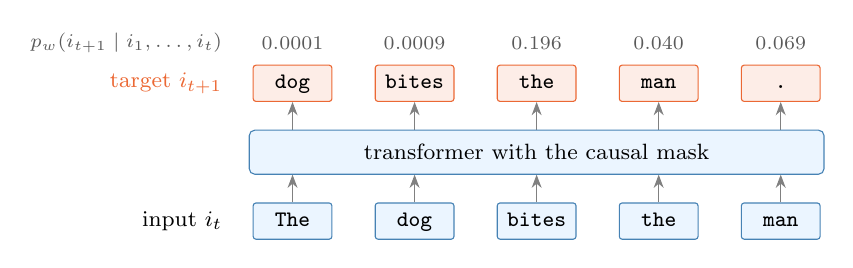
\begin{tikzpicture}[x=1.55cm, y=1mm, >=Stealth, font=\footnotesize,
    tok/.style={draw=boxframe, fill=boxbg, rounded corners=1pt, minimum height=4.6mm, minimum width=10mm,
                inner sep=1pt, font=\ttfamily\footnotesize},
    goal/.style={tok, draw=ctrl, fill=ctrl!12}]
  \foreach \t/\w/\y/\p in {0/The/dog/0.0001, 1/dog/bites/0.0009, 2/bites/the/0.196, 3/the/man/0.040, 4/man/./0.069} {
    \node[tok] (in\t) at (\t,0) {\strut\w};
    \node[goal] (out\t) at (\t,17.5) {\strut\y};
    \draw[->, black!50] (in\t.north) -- (\t,5.9);
    \draw[->, black!50] (\t,11.6) -- (out\t.south);
    \node[font=\scriptsize, text=black!65] at (\t,22.6) {$\p$};
  }
  \node[draw=boxframe, fill=boxbg, rounded corners=2pt, minimum width=7.3cm, minimum height=5.6mm] at (2,8.75)
    {transformer with the causal mask};
  \node[anchor=east, inner sep=1pt] at (-0.55,0) {input $i_t$};
  \node[anchor=east, inner sep=1pt] at (-0.55,17.5) {\ctrl{target $i_{t+1}$}};
  \node[anchor=east, inner sep=1pt, font=\scriptsize, text=black!65] at (-0.55,22.6) {$p_w(i_{t+1}\mid i_1,\dots,i_t)$};
\end{tikzpicture}

\small
\[
J(w)=-\frac1n\sum_{t=1}^{n}\log p_w\big(\ctrl{i_{t+1}}\mid i_1,\dots,i_t\big)
\]
\raggedright
The cross-entropy of lecture 04, with $|\Vocab|$ classes. The targets are the input \alert{shifted by one}: no human labels, any text is training data.
\takeaway{Thanks to the mask, one text of $n$ tokens gives $n$ training examples in one pass.}
\end{frame}


% =========================================================================
% BERT: Devlin et al. (2019), 15% of the tokens are hidden.  The two grids show which weights
% alpha_ts may be nonzero (row t, column s).
\begin{frame}{Two ways to hide the answer: GPT and BERT}
\small
\tikzset{
  tok/.style={draw=boxframe, fill=boxbg, rounded corners=1pt, minimum height=4.4mm, minimum width=8.6mm,
              inner sep=0.5pt, font=\ttfamily\scriptsize},
  goal/.style={tok, draw=ctrl, fill=ctrl!12},
  hole/.style={tok, draw=ctrl, fill=white, dashed},
}
\begin{columns}[T]
\begin{column}{0.49\textwidth}
\centering
\alert{GPT}: predict the \alert{next} token \citep{radford2018}\\[3pt]
\begin{tikzpicture}[x=9.4mm, y=1mm, >=Stealth]
  \foreach \t/\w/\y in {0/The/dog, 1/dog/bites, 2/bites/the, 3/the/man, 4/man/.} {
    \node[tok] (i\t) at (\t,0) {\strut\w};
    \node[goal] (o\t) at (\t,11) {\strut\y};
    \draw[->, black!45] (i\t) -- (o\t);
  }
\end{tikzpicture}\\[4pt]
\begin{tabular}{@{}c l@{}}
\raisebox{-0.5\height}{\maskgrid{1}} & \parbox{0.5\linewidth}{\footnotesize causal mask:\\ $t$ sees $s\le t$}
\end{tabular}

\medskip
\footnotesize
\begin{itemize}
\item every position is a training example
\item naturally \alert{writes}: sample, append, repeat
\end{itemize}
\end{column}
\begin{column}{0.49\textwidth}
\centering
\alert{BERT}: fill in the \alert{hidden} tokens \citep{devlin2019}\\[3pt]
\begin{tikzpicture}[x=9.4mm, y=1mm, >=Stealth]
  \foreach \t/\w in {0/The, 2/bites, 3/the} \node[tok] (i\t) at (\t,0) {\strut\w};
  \node[hole] (i1) at (1,0) {\strut\_\_};
  \node[hole] (i4) at (4,0) {\strut\_\_};
  \node[goal] (o1) at (1,11) {\strut dog};
  \node[goal] (o4) at (4,11) {\strut man};
  \draw[->, black!45] (i1) -- (o1);
  \draw[->, black!45] (i4) -- (o4);
\end{tikzpicture}\\[4pt]
\begin{tabular}{@{}c l@{}}
\raisebox{-0.5\height}{\maskgrid{0}} & \parbox{0.5\linewidth}{\footnotesize no mask:\\ $t$ sees both sides}
\end{tabular}

\medskip
\footnotesize
\begin{itemize}
\item $15\%$ of the tokens hidden, mostly by \texttt{[MASK]}
\item good at \alert{understanding}: each hole sees its whole context
\end{itemize}
\end{column}
\end{columns}
\takeaway{Part 2 trains a tiny BERT on Shakespeare, and makes it write by putting a \texttt{[MASK]} at the end of the text.}
\end{frame}


% =========================================================================
% Figure and samples: figures/part3_sampling.py, as in the frame "Sampling: from probabilities to
% text" of self_attention_and_transformers.tex.
\begin{frame}[fragile]{From probabilities to text: the temperature}
\small
\setlength{\abovedisplayskip}{4pt}\setlength{\belowdisplayskip}{4pt}
The model returns scores $z\in\R^{|\Vocab|}$; the next token is drawn from
\[
p_i=\frac{e^{z_i/\ctrl{\tau}}}{\sum_{j}e^{z_j/\ctrl{\tau}}},
\qquad \ctrl{\tau}\to0:\ \text{always the most likely token},\qquad \ctrl{\tau}\to\infty:\ \text{uniform}.
\]
\footnotesize GPT-2 after \texttt{Attention is all you}:

\centering
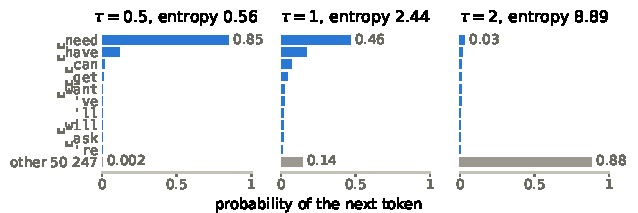
\includegraphics[width=0.9\linewidth]{sampling_temperature.pdf}

\begin{lstlisting}[style=output]
> The best way to learn mathematics is
tau=0    to learn it from a teacher.\n\nThe best way to learn mathematics is...
tau=0.7  through a teacher. You will learn how to teach, and you will learn...
tau=1.5  Hearwearill captures how in flash the Tickler microsee can portray...
\end{lstlisting}
\takeaway{Low $\tau$: safe, repetitive. High $\tau$: creative, then nonsense. Part 2: $\tau=0.8$.}
\end{frame}


% #########################################################################
% CLOSING
% #########################################################################

% =========================================================================
\begin{frame}{Summary}
\small
\begin{enumerate}
\setlength{\itemsep}{3pt}
\item \alert{History.} Attention (2014) was a help for recurrent translators. In 2017 the recurrence was removed: all tokens at once, any two one step apart.
\item \alert{Tokens.} Byte-pair encoding merges frequent pairs: frequent words whole, rare words in pieces.
\item \alert{Embedding.} A learned table, one vector per token; similar tokens end up close.
\item \alert{Self-attention.} A soft, learnable look-up: $Y=\softmax\big(QK^\top/\sqrt{d_a}\big)V$. The $\sqrt{d_a}$ keeps the softmax from freezing.
\item \alert{Order.} Attention is permutation equivariant; the positions $p_t$ and the causal mask bring the order in.
\item \alert{Training.} The text is its own label: predict the next token (GPT) or the hidden one (BERT), and minimize the cross-entropy.
\end{enumerate}
\end{frame}


% =========================================================================
% Timing: the notebook run top to bottom with nbconvert, November 2026: on a 14-core CPU 137 s in
% all (the training cell of section 6: 119 s; generation: 7 s; everything else under 4 s); with
% OMP_NUM_THREADS=4, as on a laptop, the training cell takes 133 s.
\begin{frame}{Part 2: the notebook}
\small
\texttt{notebooks/archive/06\_transformers\_old.ipynb}: each section is a slide of today.

\medskip
\footnotesize
\renewcommand{\arraystretch}{1.25}
\begin{tabularx}{\textwidth}{@{}c l >{\raggedright\arraybackslash}X@{}}
\toprule
\textbf{\S} & \textbf{Notebook} & \textbf{Slides} \\
\midrule
1 & self-attention in five lines & self-attention; soft look-up \\
2 & why $1/\sqrt{d_a}$ & the softmax freezes without it \\
3 & multi-head attention & several look-ups in parallel \\
4 & positional encoding & attention does not see the order; positions \\
5 & the transformer block & residual, LayerNorm, MLP \\
6 & a tiny BERT on Shakespeare & self-supervised learning; GPT and BERT; temperature \\
\bottomrule
\end{tabularx}

\medskip
\small
\alert{Run time} on a CPU: about \alert{2--3 minutes} for the whole notebook, almost all of it the training in \S6 (2000 steps, $10^5$ parameters).
\takeaway{Start the training cell of \S6 first, and read \S1--5 while it runs.}
\end{frame}


% =========================================================================
\begin{frame}[allowframebreaks]{References}
\tiny
\nocite{rush2018,huang2022}
\bibliographystyle{plainnat}
\bibliography{self_attention_and_transformers_part1}
\end{frame}

\end{document}
